\section{Current Measurements Synchronization}
Section \ref{sec:INA238} described the very detailed view of INA238/INA2xx sensors, the essence of explaining INA is the most competitive solution for current measurements and it is the main pillar in this project to acquire current measurements and other several measurements(Shunt Voltage, Bus Voltage, ALERT). Among all measurements synchronizing the current measurements is the nail hitting. The following sections will brief different approaches to synchronize the current measurements.

\subsection{Simultaneous Write and Sequential Read :}
Thanks to the INA238/INA2xx multi-addressing functionality \cite[p.18]{INA238_User_Datasheet}, INA operates through I2C and the address of the INA can be configured by address lines A0 and A1 pulling to Vdd or GND. Figure \ref{fig:INA2xx_Simultaneous_Write_and_Sequential_Read}shows the Simultaneous Write and Sequential Read approach. Configure all the INAs (Write Control register) simultaneously by keeping all the INA addresses the same. Address configuration can be done, by the controller. As soon as write is done all the INAs start current acquisitions and report measurements at the same instant. For reading the current measurements, configure sensor address lines to different addresses(for instance 0x40,0x41,0x44,0x44, and so on) and read current measurements sequentially from each  INA.

\begin{figure}
    \centering
    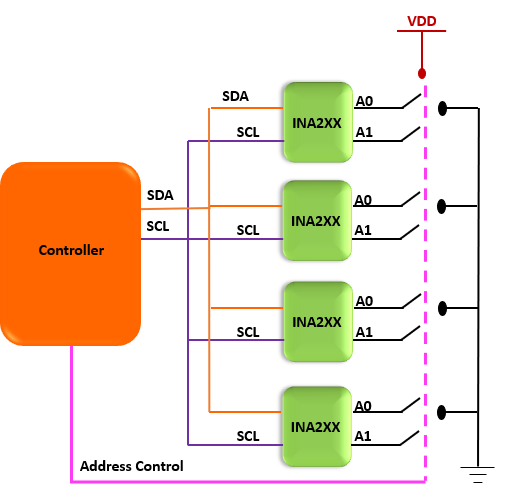
\includegraphics[width=0.4\textwidth]{Chap05/Figures/INA_MultiWrite.PNG}
    \caption{INA2xx Simultaneous Write and Sequential Read}
    \label{fig:INA2xx_Simultaneous_Write_and_Sequential_Read}
\end{figure}

"Simultaneous Write and Sequential Read" \ref{fig:INA2xx_Simultaneous_Write_and_Sequential_Read} approaches are reliable only for low precision and sequential data storage applications. SoC estimation is dealing with real-time current flowing in the battery, let's say a case where we write all sensors at the same time parallelly by considering the acknowledgment but this acknowledge could be sent by any one of the sensors if any one sensor dropped in between writing the data (configuring) controller can not differentiate. The controller only gets to know the sensor is not configured or dropped after it samples the first current data. Unfortunately, by that time the battery balancing might have already started if we do not receive current measurement data from anyone's sensor we might be in deep trouble. Simultaneous Write and Sequential Read are simple to implement but it is not robust and reliable for BMS applications.

\subsection{Synchronizing by Delayed Measurements  }
Depending on the MODE bits that have been specified and set in the ADC CONFIG register, the INA238 can measure the shunt voltage, bus voltage, die temperature, or any combination of these. This enables the user to further tune the monitoring function to meet the demands of the particular application by choosing modes to convert simply the shunt voltage or bus voltage.
\begin{figure}
    \centering
    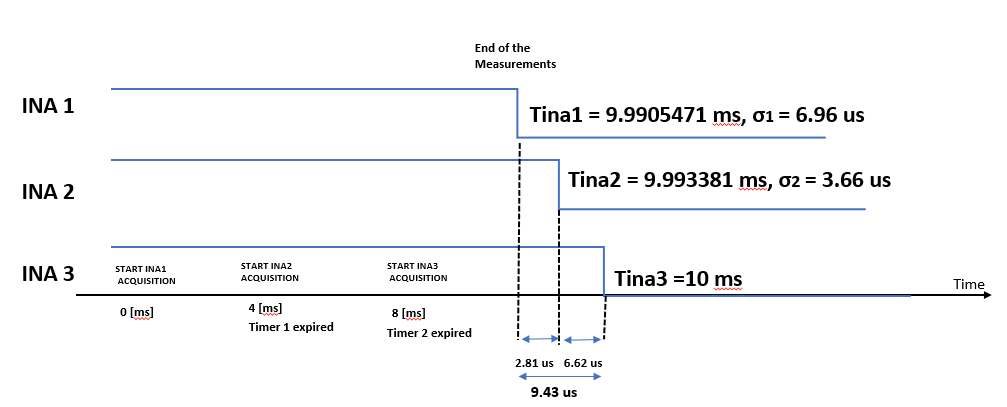
\includegraphics[width=0.9\textwidth]{Chap05/Figures/INA_synchronization_alert.PNG}
    \caption{INA2xx Delayed Synchronization}
    \label{fig:INA_synchronization_alert}
\end{figure}

The INA238 conversion can be delayed to synchronize with other system components by setting the CONVDLY bits in the CONFIG register to a value between 0 (no delay) and 510 ms. The conversion delay resolution in programming is 2 ms. By default, the conversion delay is set to 0.As soon as the measurement conversion is complete the INA2xx ALERT pin asserts. Figure \ref{fig:INA_synchronization_alert} shows synchronizing the 3 sensors by writing the sequential delay for instance first sensor has a conversion delay of 2ms subsequently adding other sensors' conversion delay (INA1 delay = INA2 delay + INA3 delay + 2ms ). At the end of the 10ms all the sensors sample at the same time, finish the conversion and assert the alert pin.  As soon as the ALERT is asserted the controller interrupts will trigger and the controller will read the data from the sensors sequentially. The point here is not reading the data sequentially or parallel important is all the sensors must sample the current at the same instance time.

\paragraph{Implementation of Synchronizing by Delayed Measurements Algorithm:}\label{sec:INA2XX_synch_delayed_method}
\begin{itemize}
    \item Send to three INAs: the config alert command (bit 14, register Bh) and sets the CONVDLY (bits 13-6 register 0h), which is the delay for initial ADC conversion. ​
    \item When START ACQUISITION command is sent, the INA waits the time specified by CONVDLY ​before starting the conversion.​
    \item CONVDLY INA 1 = 10 ms, ​CONVDLY INA 2 = 6 ms, ​CONVDLY INA 3 = 2 ms​
    \item Two Timers are used to send the start acquisition command: Timer 1 = 4ms, Timer 2 = 4ms​
    \item As two timers finish writing controller wait for ALERT interrupt to read data from sensors
\end{itemize}

Figure \ref{fig:INA_synchronization_alert} shows the three INAs synchronize current measurement current, each INA triggered with a different delay to acquire data at the end of 10ms all the INAs are asserted alert signals. The sque of the ALERT of the INAs is quite impressive because they have responded with arround 10us of sque.

So on and so forth the above sections briefed about the current sensor, features, and synchronizing methods. This section will put a more detailed view of one of the current measurement applications from BMS architecture, Power analyzer emulation, and current measurement synchronization.

\section{Balancing Current Measurement}

As discussed in chapter \ref{ch:Architecture_Active_Balancing_BMS} active balancing architecture \ref{fig:BMS Architecture}the controller will operate the DC/DC converter either in buck or boost mode depending on the unbalanced node. The output current of the DC/DC converter is the total balancing current that needs to flow from the battery node to the pack or vice versa. DC/DC converter input and output both have the shunt resistor \ref{fig:BMS Architecture} where INAs are coupled with them to measure the current. 
All the currents in the architecture \ref{fig:BMS Architecture} are measured with the power analyzer setup as briefed in chapter \ref{fig:Battery_Pack_modeling_Architec},\ref{algo:PowerAnalyzer_Modeling}(Measurement view), and all the INAs synchronized with the "INAs delayed measurement algorithm" approach as mentioned in section \ref{sec:INA2XX_synch_delayed_method}. Though, we have several currents(Charging/Discharging TOP and bottom current, DC/DC converter low and high side currents) to talk about in the architecture \ref{fig:BMS Architecture} I would like to stress the DC/DC output current more! \ref{fig:Battery_Balancing_Current}. 
Because the output current of the DC/DC converter is the balancing current that can flow from the battery node to the battery pack or vice versa, which is one of the main currents that determine the battery SOC(charging and discharging excluded in this example). 
As the balancing current reaches the threshold current (shunt current threshold set by the user Figure \ref{fig:Battery_Balancing_Current}) ALERT will be asserted by the sensor (Section \ref{sec:INA238})  and the controller will monitor the DC/DC output shunt resistor current sensor and drop the balancing current below the threshold and maintains the same current until the balancing timer period ends. 

\begin{figure}
    \centering
    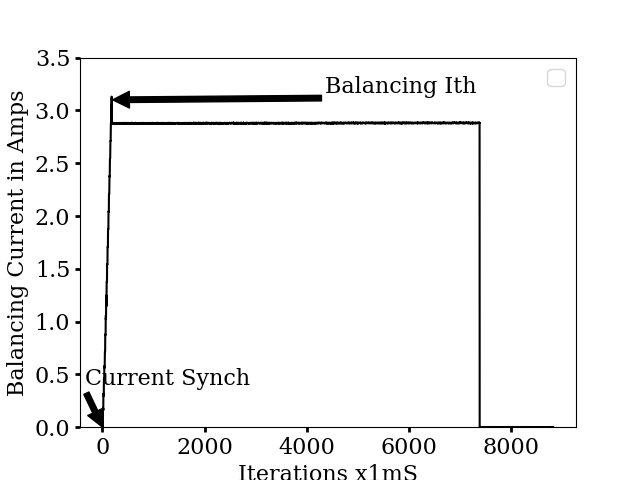
\includegraphics[width=0.6\textwidth]{Chap05/Figures/ShuntCurrent.png}
    \caption{Battery Balancing Current}
    \label{fig:Battery_Balancing_Current}
\end{figure}